\begin{minipage}[t]{180mm}
\fcolorbox{black}{white}{
\begin{minipage}[b]{30mm}

\includegraphics[width=0.5\linewidth]{unflogo.pdf}
\end{minipage}
\begin{minipage}[b]{100mm}
\Huge \textbf{UNF NEWZ} \\
\Large -- Søvn og retsstavning er overvurderet! 
\end{minipage}
\begin{minipage}[b]{50mm}
\Large Onsdag 17.07.2015 \\
\normalsize Redigeret i \LaTeX\ af \\ SOM, MGS, MMN, SABH
\end{minipage}
}
\end{minipage}



\begin{minipage}[b]{0.95\linewidth}
\begin{minipage}[t]{0.47\textwidth}
\vspace{3mm}

\section*{Velkomst}
Kære subjekter,

deltagelse på UNF Matematik Camp har siden 2007 vist sig at have en positiv effekt på optagelsen på de naturvidenskabelige uddannelser for deltagerne. Dette er for den samfundsøkonomiske udvikling et meget positiv tiltag. Analyserne har også vist, at de deltagere som arbejder hårdest og sover mindst senere klarer sig bedst på deres uddannelse, om det er som økonom eller som skarpretter. Og da nationaløkonomiske interesser overskygger alle andre hensyn, vil vi her på Matematik Camp arbejde så effektivt så muligt, uden unødvendige regler eller demokrati. Der vil blive afsat $18$ til $24$ timer dagligt til hård matematisk træning. For at opnå optimalt makroøkonomisk udbytte vil deltagere, hvis effektivitet kommer under $\max(\text{median},\text{middelværdi})$ vil blive hjemsendt på egen regning. Dette kommer fra det kendte økonomiske data, som dokumenterer at alle mennesker burde aflives når de fylder $70$ år, som den ultimative gave fra dem til samfundet. Deltagere, som ikke er klar på at yde det ypperste for samfundet i den anden ende kan lige så godt tilslutte sig de $70$-årige. Alt hensyntagen til individer er for ledelsen på Matematik Camp total uvedkommende og futilt. 

Det vil være mig en ære at hjælpe jer alle på vej mod storhed for vores verdensøkonomi, og for vores allesammens bedste, og den uge jeg har fået til denne opgave vil blive udnyttet for at opnå maksimal effektivitet!

God arbejdslyst 

{\flushright\emph{1. co-koordinator, Helene, næsten cand. scient. stat.-oecon.}}

\section*{Velkomst}
Kære kammerater,

I er nu på vej på en åndelig rejse mod mere medmenneskelighed og et tættere forhold til jeres aksiomatiske rødder. Maximen på denne lejr vil være, i respektful diskurs, at modstå døden der ligger i stilheden og opsuge i vores hjerter, det liv der ligger i strømmen. 

Establishementet, har påtvunget mig en forældet ledelsesrolle, men denne vil vi hurtigt dekonstruere i lejrens post-hierakiske rundkredskultur. Hver morgen vil dagens foretrukkende pålægschokoladefarve fastlægges i følelsesbetonede diskutioner, og vi vil først spise i fællesskab når konsensus om den farve hjertet slår får dén dag er nået. Selvfølgelig vil vi aldrig enedes om at fortrække den lyse farve, da dette ville understøtte fordomme om livet på solskinsøen, det mørke derimod ville støtte op om den forældelde identifikation med det mørke Jylland. 

Dette åbenlyse skisma, skader dog ikke, da morgenmad i sagens natur er et levn fra industrialiseringens stændersamfund som prøvede at påtvinge proletariatet afstumpede mekaniserede livsomstændigheder og afskære dem fra naturens cykler. Og med nok kærlighed vil vi sagtens kunne leve på fællessang alene i en uge.

Empirien truer fra nord, og militarismen fra øst, men frygt ej, jeg vil til en hver tid ofre jeres liv for at opretholde glæden i min mave. 

{\flushright\emph{Den ligeste blandt lige, cokoordinator, Morten Agger}}

\end{minipage}
\hfill\begin{minipage}[t]{0.47\textwidth}

\vspace{1mm}
\tikzstyle{mybox} = [draw=white, fill=blue!20, very thick,
    rectangle, rounded corners, inner sep=10pt, inner ysep=20pt]
\tikzstyle{fancytitle} =[fill=red, text=white]

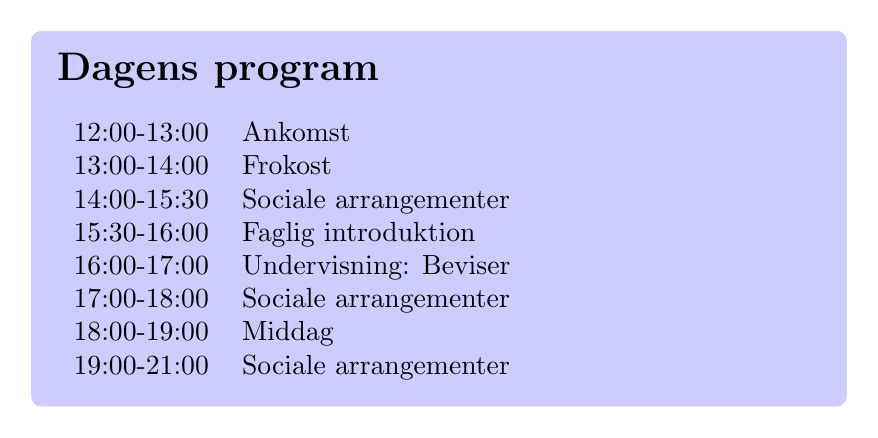
\begin{tikzpicture}
\node [mybox] (box){%
\begin{minipage}{0.80\textwidth}
\vspace{-4mm}\section*{Dagens program}
\begin{tabular}{ll}
12:00-13:00 & Ankomst \\
13:00-14:00 & Frokost \\
14:00-15:30 & Sociale arrangementer \\
15:30-16:00 & Faglig introduktion \\
16:00-17:00 & Undervisning: Beviser \\
17:00-18:00 & Sociale arrangementer \\
18:00-19:00 & Middag \\
19:00-21:00 & Sociale arrangementer \\
\end{tabular}
\vspace{-4mm}
\end{minipage}
};
\end{tikzpicture}%

\section*{Velkommen til Matematik Camp!}
Deltagere!\\
Det er jer en ære at blive budt velkommen af mig til syv døgn under min kompetente kommando! I disse døgn vil i udvikle jer til stærkere og mere disciplinerede mennesker, der ikke bare bliver mere stringente matematikere og lære at marchere frem langs nye metriker, i vil lære fast takt og tone og hvordan rigtige personer opfører sig. For at opfylde dette yderlige mål har jeg i år bestemt at der tilføjes et par simple regler som I, som underornede deltagere, skal overholde. For det første vil det på årets Matematik Camp ikke være tilladt at stå eller sidde i rundkreds, da dette er yderst uhøfligt over for firkanter. Af andre simple regler skal der nævnes at, når man starter med at gå skal der altid startes med venstre ben, farven blå er bandlyst, længerevarende øjenkontakt er strengt forbudt og folk der går stik øst vil blive bortvist. Målet med disse traditionelle regler er at assimilere alle jer uslebne små pjok ind til en hærdet hær af unge matematikere. Deltagere, som ikke kan overholde disse simple og let opfyldte regler vil blive tvunget til at skrive haikudigte, indtil de forløses af sultedøden. Til slut vil jeg gerne endnu en gang byde jer alle sammen velkommen, yderdørene er allerede låste og vil tidligst blive låst op lørdag eftermiddag, og jeg vil dedikere hver en time jeg har indtil da på at få jer formet som sande matematikere.

{\flushright\emph{Jeres koordinator, Morten Grue Sørensen}}

\begin{center}
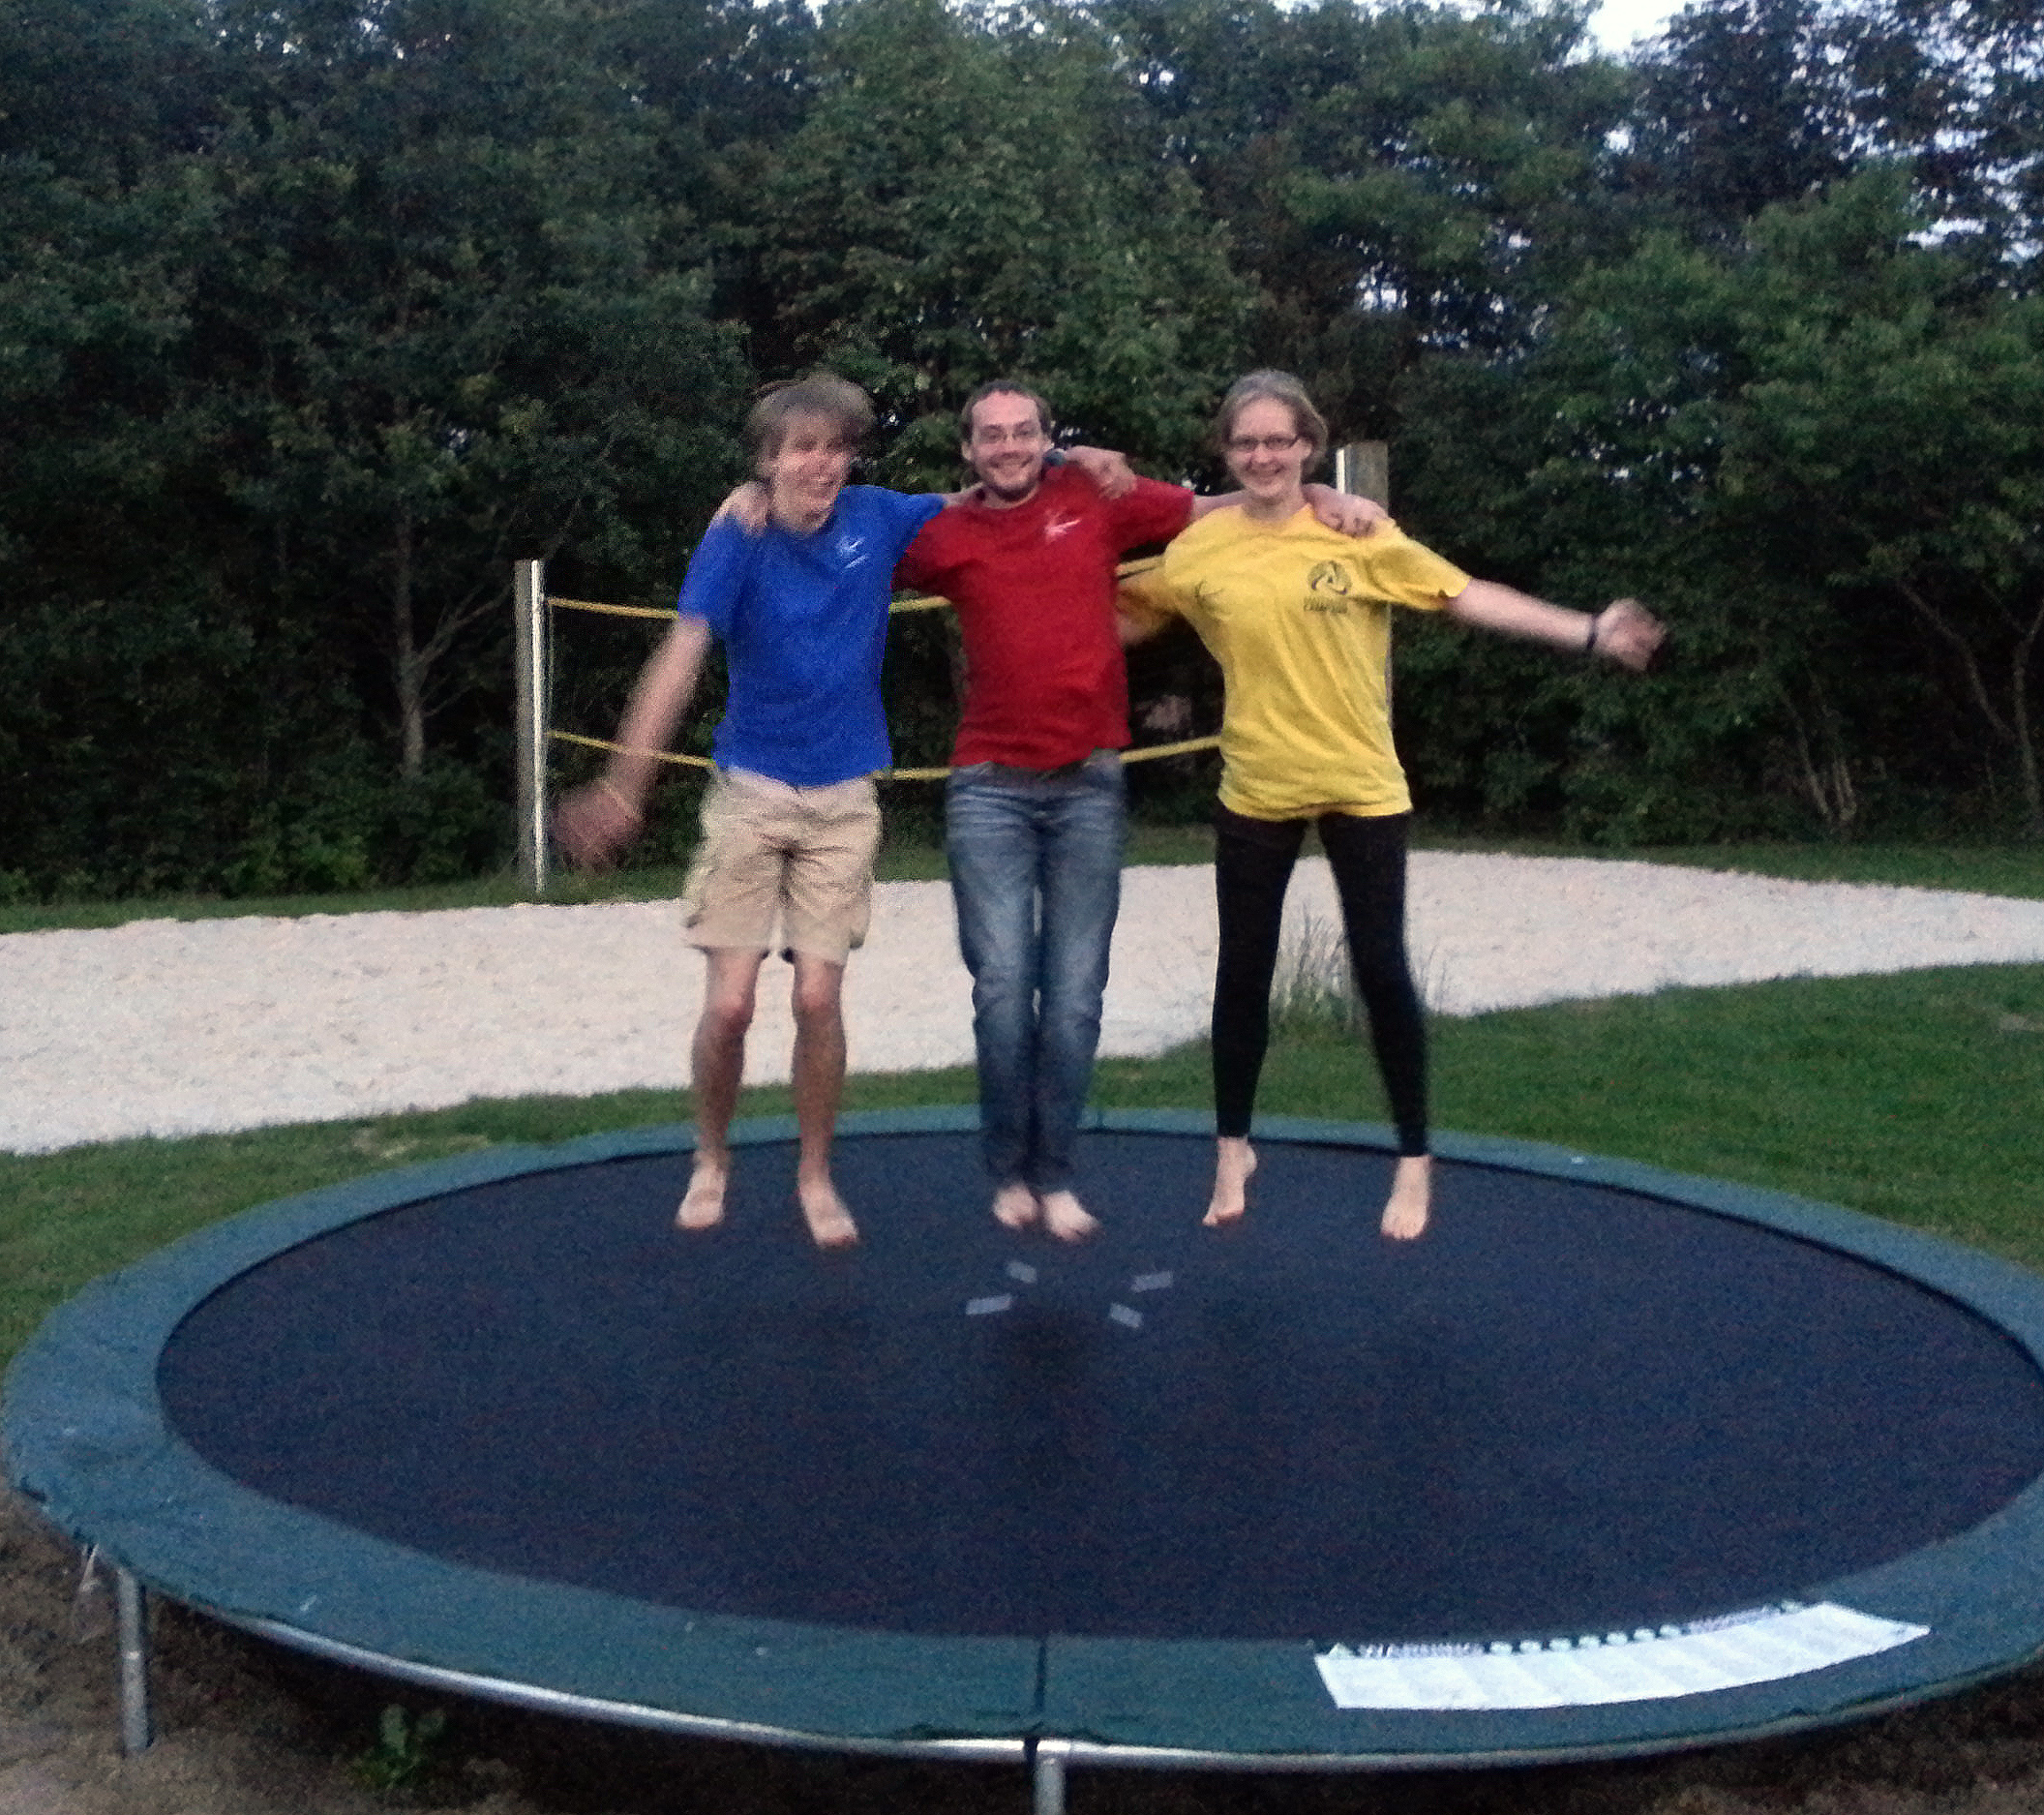
\includegraphics[width=\linewidth]{koordinatorer2.jpg}
\end{center}

\end{minipage}
\end{minipage}
